\documentclass[11pt]{article}

% ---------- packages ----------
\usepackage[utf8]{inputenc}
\usepackage[T1]{fontenc}
\usepackage[margin=1in]{geometry}
\usepackage{amsmath,amssymb}
\usepackage{natbib}
\usepackage{graphicx}
\usepackage{booktabs}
\usepackage{caption}
\usepackage{enumitem}
\usepackage{authblk}
\usepackage[hidelinks]{hyperref}
\usepackage{xcolor}
\usepackage{titlesec}

\captionsetup{font=small,labelfont=bf}
\titleformat{\section}{\large\bfseries}{\thesection}{0.6em}{}
\titleformat{\subsection}{\normalsize\bfseries}{\thesubsection}{0.6em}{}
\setlength{\parskip}{0.35em}
\setlength{\parindent}{0pt}

% ---------- title ----------
\title{\textbf{Does Music's Sensitive Period Leave a Trace in\\
Episodic Memory's White Matter?}\\[0.3em]
\large A Graph-Theoretic Test of the Chicken-and-Egg Problem Using HCP-D}

\author[ ]{20230340 Yeseul Seo }
\affil[ ]{\texttt{github.com/ashleysys04-blip/music\_connectome\_pipeline}}
\affil[ ]{Department of Brain \& Cognitive Sciences, KAIST}
\date{BCS499 Final Report}

\begin{document}
\maketitle

% ==================================================================
\begin{abstract}
\noindent
Early music training is widely believed to enhance children's cognitive development, but the underlying causal story remains contested. Three competing explanations have shaped the literature: a \emph{sensitive-period} account (when training starts matters), a \emph{dose-response} account (how much one trains matters), and a \emph{skeptical} account (apparent effects reduce to confounding). I used HCP-D data ($N=473$ with usable structural connectomes; trained-only $n\approx183$) to test these scenarios on episodic memory, operationalized via the Picture Sequence Memory (PSM) task. Music onset age and cumulative log-hours of training were entered into a single multiple regression (M3) so their partial effects could be compared on a common scale. Across 11 graph-theoretic features of the white-matter connectome (global efficiency, modularity, small-worldness, characteristic path length, and within/between-network strength for DMN, FPN, and MTL), only small-worldness reached nominal significance with PSM ($\beta=+0.13$, raw $p=0.019$; FDR n.s.). The music-side results showed a textbook \emph{suppressor pattern}: onset's partial coefficient grew from $\beta=-0.092$ in M1 to $\beta=-0.207$ in M3 once cumulative hours was controlled, while hours' partial effect remained smaller in magnitude ($\beta=-0.158$). Bootstrap mediation across all 11 brain features yielded no indirect effects (all 95\% CIs included zero). Together, the data lean toward the sensitive-period scenario in direction and effect-size ordering, but neither $\beta$ reached $p<0.05$, and the absence of mediation implies that---if a sensitive-period effect exists in HCP-D---it does not travel through macroscale white-matter topology.
\end{abstract}

% ==================================================================
\section{Background and Significance}
My motivation for this project began with a common parental intuition: that early musical exposure makes children smarter. Many parents enroll their children in piano lessons before elementary school, hoping the experience will sharpen the brain. The popular literature reinforces this idea, but the empirical literature does not speak with one voice. Whether music training causally improves general cognition has been debated for decades, and the debate has the structure of a chicken-and-egg problem.

Three positions occupy this debate. First, the \textbf{sensitive-period view} holds that the timing of training matters, that the developing brain has a window during which musical experience can sculpt neural circuitry in ways that mature brains cannot. \citet{steele2013} provided the classic evidence: white-matter integrity in the posterior corpus callosum was systematically related to whether musicians began training before or after age seven, even after matching for total hours. Second, the \textbf{dose-response view} holds that the apparent onset effect is really an hours effect: children who start earlier accumulate more total practice by adulthood, and that cumulative dose is what matters, not the calendar age at first lesson \citep{schellenberg2020}. Third, the \textbf{skeptical view} holds that neither variable carries information once one properly controls for the confounding effects of socioeconomic status, family environment, and pre-existing aptitude \citep{sala2017}.

These three positions cannot be distinguished by simple correlation. Because onset age and cumulative hours are strongly negatively correlated, the relationship of either with cognition is ambiguous. The natural arbiter is a multiple regression that includes both predictors: the partial coefficients on onset and hours, holding the other constant, directly test which scenario fits the data. This is the analytic strategy this project pre-registered.

Episodic memory is a particularly appropriate behavioral outcome. Music learning is fundamentally sequential. Practice consists of encoding ordered temporal patterns, remembering motor sequences, and binding melodic events to contextual cues. The NIH Toolbox Picture Sequence Memory (PSM) task probes this same machinery: participants reproduce ordered sequences of pictured events. Compared with the broad construct of ``intelligence,'' PSM offers a concrete, well-validated, theoretically motivated dependent variable that is available across all HCP-D participants. For this reason, PSM was selected as the primary cognitive outcome rather than as a proxy for general intelligence.

The white-matter side of the question is motivated by recent connectome-level work showing that structural network topology is itself developmentally dynamic. \citet{mousley2025} reported four major lifespan turning points in white-matter topology (ages 9, 32, 66, and 83) and identified small-worldness as the strongest LASSO-retained predictor of age in the 9--32 epoch, the very epoch that contains the HCP-D age range. If music's sensitive period writes itself into the connectome, this is the developmental window in which we would expect that trace to be detectable.

This study addresses a scientifically meaningful question in developmental neuroscience: how early musical training is related to episodic memory development and whether this relationship is reflected in structural brain connectivity. Despite decades of research on music training and cognition, two important problems remain unresolved. First, there is an identification problem. Because onset age and cumulative training hours are intrinsically correlated, earlier starters tend to accumulate more practice, and their effects on cognition are often confounded. Studies that control for training hours through matching can reduce some group differences, but they cannot directly compare onset age and cumulative practice as competing predictors. This project addresses this gap by estimating their partial effects within a joint model, thereby testing whether training onset explains memory outcomes beyond total training exposure. Second, there is an explanatory-level problem. The cognitive benefits of music training have been reported predominantly at the behavioral level, whereas whether such effects are reflected in the structural organization of the connectome remains less clear, particularly for episodic memory. By linking behavioral memory performance to white-matter network features through mediation analysis, this study asks not only whether an association exists, but also at which neural level it may reside. Moreover, the project targets sequential episodic memory, a theoretically matched cognitive outcome for musical experience, rather than relying on diffuse measures of general intelligence transfer. Beyond its theoretical contribution, the study has practical relevance for the design of early-childhood enrichment, as it may help clarify how caregivers and educators should think about the timing and allocation of developmental resources across the early years.

% ==================================================================
\section{Research Questions and Hypotheses}

\subsection{Research questions}
\textbf{RQ1.} Is music onset age associated with PSM performance? Does the association survive controlling for cumulative training hours?

\textbf{RQ2.} Is music onset age associated with white-matter network organization? If a behavioral effect exists, is it mediated by these network features?

\subsection{Models}

The first model tested the sensitive-period hypothesis by including only music onset age:
\[
\mathrm{M1:}\quad
\mathrm{PSM}_i
=
\beta_0
+
\beta_1 \mathrm{Onset}_i
+
\beta_2 \mathrm{Age}_i
+
\beta_3 \mathrm{Sex}_i
+
\beta_4 \mathrm{WISC}_i
+
\epsilon_i.
\]

The second model tested the dose-response hypothesis by including only cumulative training hours:
\[
\mathrm{M2:}\quad
\mathrm{PSM}_i
=
\beta_0
+
\beta_1 H_i
+
\beta_2 \mathrm{Age}_i
+
\beta_3 \mathrm{Sex}_i
+
\beta_4 \mathrm{WISC}_i
+
\epsilon_i.
\]

The third and primary model included both onset age and log-hours simultaneously:
\[
\mathrm{M3:}\quad
\mathrm{PSM}_i
=
\beta_0
+
\beta_1 \mathrm{Onset}_i
+
\beta_2 H_i
+
\beta_3 \mathrm{Age}_i
+
\beta_4 \mathrm{Sex}_i
+
\beta_5 \mathrm{WISC}_i
+
\epsilon_i.
\]
This model was central because onset age and cumulative training hours are naturally correlated: individuals who begin earlier often accumulate more total practice. By including both predictors in the same model, M3 tested whether earlier onset explained unique variance in PSM beyond training amount, and whether training amount explained unique variance beyond onset age.

The fourth model added an interaction term:
\[
\mathrm{M4:}\quad
\mathrm{PSM}_i
=
\beta_0
+
\beta_1 \mathrm{Onset}_i
+
\beta_2 H_i
+
\beta_3 \left(\mathrm{Onset}_i \times H_i\right)
+
\beta_4 \mathrm{Age}_i
+
\beta_5 \mathrm{Sex}_i
+
\beta_6 \mathrm{WISC}_i
+
\epsilon_i.
\]
This interaction model tested whether the effect of starting age depended on the amount of training. The trained-only sample size for this step was approximately $n=183$.

\subsection{Pre-registered scenarios}
The central behavioral question was whether PSM is better explained by the age at which music training began or by the cumulative amount of training. This comparison was tested in the primary joint model, M3, in which onset age and cumulative training hours were entered simultaneously:
\begin{equation*}
\mathrm{PSM} \;\sim\; \beta_1\cdot \mathrm{onset\_age} \;+\; \beta_2\cdot \log(\mathrm{hours}) \;+\; \mathrm{covariates}
\end{equation*}
Here, a larger onset value means later music onset, whereas a larger hours value means greater cumulative training. Therefore, a sensitive-period account predicts a negative onset coefficient: later onset should be associated with lower PSM. By contrast, a pure dose-response account predicts a positive hours coefficient: greater cumulative training should be associated with higher PSM.

The three competing scenarios were therefore defined as follows:
\begin{itemize}[leftmargin=1.4em,itemsep=2pt]
  \item \textbf{H1a (Sensitive period):} $|\beta_1| > |\beta_2|$, with $\beta_1 < 0$.
  The timing of music onset should be the stronger predictor of PSM.
  \item \textbf{H1b (Dose-response):} $|\beta_2| > |\beta_1|$, with $\beta_2 > 0$.
  The cumulative amount of music training should be the stronger predictor of PSM.
  \item \textbf{H1c (Skeptical):} $\beta_1\approx 0$, $\beta_2\approx 0$, both coefficients are approximately zero after covariate adjustment.
  Any apparent music-training effect should disappear once confounders are controlled.
\end{itemize}

% ==================================================================
\section{Methods}

\subsection{Step 1: Dataset and sample construction}
Data come from the Human Connectome Project---Development (HCP-D). The starting demographic table contained 652 participants. Music variables were merged from the NDA SAIQ instrument (500 participants, 286 ever-trained). Cognitive variables (PSM, Flanker, DCCS, list sorting, pattern comparison) were merged from the corresponding NIH Toolbox files (611 participants with at least one cognitive score). After requiring a non-missing PSM score, 473 participants remained, all of which had usable structural connectivity matrices after quality control.

\subsection{Step 2: Music variables}
Music onset age was estimated as the participant's current age minus their reported total years of training. Participants reporting no training were treated as untrained and excluded from the trained-only analyses. Cumulative hours was estimated from the reported years $\times$ weeks/year $\times$ days/week $\times$ minutes/session, then log-transformed to compress the heavy right tail and stabilize variance.

\subsection{Step 3: Structural connectomes and graph metrics}

For each participant, the structural connectome was represented as a weighted undirected matrix
\[
S \in \mathbb{R}^{246 \times 246},
\]
reconstructed from HCP-D diffusion MRI using DSI Studio's QSDR pipeline on the Brainnetome atlas. The raw edge weights corresponded to streamline counts. Before graph construction, each matrix was symmetrized and its diagonal was removed:
\[
W^{(0)}_{ij} =
\begin{cases}
\frac{1}{2}\left(S_{ij}+S_{ji}\right), & i \neq j,\\
0, & i=j.
\end{cases}
\]
Because streamline counts were highly right-skewed, edge weights were stabilized with a log transform:
\[
W^{(\log)}_{ij}
=
\log\left(1+\max\left(W^{(0)}_{ij},0\right)\right).
\]

For the global graph-theoretic metrics, matrices were proportionally thresholded. For a density level $\rho$, the number of retained undirected edges was
\[
K_{\rho}
=
\mathrm{round}\left(
\rho \frac{N(N-1)}{2}
\right),
\]
where $N=246$. The set $E_{\rho}$ contained the $K_{\rho}$ strongest off-diagonal edges in the upper triangle of $W^{(\log)}$. The thresholded matrix was therefore
\[
W^{(\rho)}_{ij} =
\begin{cases}
W^{(\log)}_{ij}, & \{i,j\}\in E_{\rho},\\
0, & \text{otherwise}.
\end{cases}
\]
The primary density was $\rho=0.15$, with robustness checks at $\rho=0.10$ and $\rho=0.20$. After thresholding, weights were normalized by the maximum retained weight:
\[
A^{(\rho)}_{ij}
=
\frac{W^{(\rho)}_{ij}}
{\max_{u,v} W^{(\rho)}_{uv}},
\]
so that all nonzero edge weights lay in $[0,1]$. All subsequent global graph metrics were computed on this weighted undirected matrix $A^{(\rho)}$.

Node strength was defined as the weighted degree
\[
s_i
=
\sum_{j=1}^{N} A_{ij},
\]
and total strength was computed as the sum of all upper-triangular edge weights:
\[
S_{\mathrm{total}}
=
\sum_{i<j} W^{(\log)}_{ij}.
\]

Global efficiency was computed as the average inverse shortest-path distance between all node pairs:
\[
E_{\mathrm{glob}}
=
\frac{1}{N(N-1)}
\sum_{i\neq j}
\frac{1}{d_{ij}},
\]
where $d_{ij}$ is the length of the shortest weighted path between nodes $i$ and $j$. To convert connection weights into path lengths, stronger connections were treated as shorter distances:
\[
\ell_{ij}
=
\begin{cases}
1/A_{ij}, & A_{ij}>0,\\
\infty, & A_{ij}=0.
\end{cases}
\]
The shortest-path distance was therefore
\[
d_{ij}
=
\min_{p:i\rightarrow j}
\sum_{(u,v)\in p}
\ell_{uv}.
\]

Characteristic path length was computed from the same shortest-path distance matrix:
\[
L
=
\frac{1}{N(N-1)}
\sum_{i\neq j} d_{ij},
\]
excluding disconnected node pairs when distances were infinite. Thus, both global efficiency and characteristic path length reflect a shortest-path communication model, where information is assumed to travel along the strongest and shortest available routes in the structural network.

The weighted clustering coefficient was computed at the node level and then averaged across nodes:
\[
C
=
\frac{1}{N}
\sum_{i=1}^{N} C_i.
\]
For each node $i$, $C_i$ quantified the tendency of its neighbors to also be connected to each other, weighted by the geometric mean of triangle edge weights:
\[
C_i
=
\frac{
\sum_{j,k}
\left(A_{ij}A_{ik}A_{jk}\right)^{1/3}
}{
k_i(k_i-1)
},
\]
where $k_i$ is the number of nonzero neighbors of node $i$. This measure is high when a node participates in strongly weighted local triangles.

Modularity was computed by partitioning the graph into communities and maximizing the quality function
\[
Q
=
\frac{1}{2m}
\sum_{i,j}
\left[
A_{ij}
-
\frac{s_i s_j}{2m}
\right]
\delta(g_i,g_j),
\]
where
\[
m
=
\frac{1}{2}
\sum_{i,j} A_{ij},
\]
$s_i$ and $s_j$ are node strengths, $g_i$ and $g_j$ are the community labels of nodes $i$ and $j$, and $\delta(g_i,g_j)=1$ if the two nodes belong to the same community and $0$ otherwise. Larger $Q$ indicates stronger separation into within-community connections relative to what would be expected from node strength alone.

Small-worldness was computed by comparing the observed network's clustering and path length to degree-preserving randomized null networks:
\[
\sigma
=
\frac{C/C_{\mathrm{rand}}}{L/L_{\mathrm{rand}}},
\]
where $C$ and $L$ are the observed mean clustering coefficient and characteristic path length, and $C_{\mathrm{rand}}$ and $L_{\mathrm{rand}}$ are their averages across randomized networks. The randomized networks preserved the degree sequence while rewiring edges, providing a null model for the expected clustering and path length of a network with comparable degree structure. A value $\sigma>1$ indicates a network with greater local clustering than a comparable random graph while maintaining relatively short path lengths.

In addition to global graph metrics, hypothesis-driven network-level connection strengths were computed for three Yeo-defined subnetworks: the default mode network (DMN), frontoparietal network (FPN), and medial temporal/limbic network (MTL). Unlike the global graph metrics, these within- and between-network features were computed from the full log-transformed SC matrix rather than the proportionally thresholded matrix. To remove participant-level multiplicative scaling effects, the full log-transformed matrix was normalized by its maximum edge weight:
\[
\widetilde{W}_{ij}
=
\frac{W^{(\log)}_{ij}}
{\max_{u,v} W^{(\log)}_{uv}}.
\]
For a network $R$ with node set $V_R$, within-network strength was defined as the mean normalized edge weight among all pairs of nodes inside that network:
\[
\mathrm{Within}(R)
=
\frac{2}{|V_R|(|V_R|-1)}
\sum_{\substack{i<j\\ i,j\in V_R}}
\widetilde{W}_{ij}.
\]
For two distinct networks $R$ and $T$, between-network strength was defined as
\[
\mathrm{Between}(R,T)
=
\frac{1}{|V_R||V_T|}
\sum_{i\in V_R}
\sum_{j\in V_T}
\widetilde{W}_{ij}.
\]
This yielded six network features:
\[
\mathrm{DMN}_{\mathrm{within}},\quad
\mathrm{FPN}_{\mathrm{within}},\quad
\mathrm{MTL}_{\mathrm{within}},
\]
\[
\mathrm{DMN}\text{-}\mathrm{FPN}_{\mathrm{between}},\quad
\mathrm{DMN}\text{-}\mathrm{MTL}_{\mathrm{between}},\quad
\mathrm{FPN}\text{-}\mathrm{MTL}_{\mathrm{between}}.
\]

Together, the graph metrics captured global integration, local segregation, community structure, and small-world organization, while the network-level features captured anatomically motivated connection strengths among memory- and control-related subnetworks. More decentralized communication models, such as greedy navigation, random walks, diffusion, or communicability, were not modeled in the present analysis.


\subsection{Statistical models}

All confirmatory analyses were conducted using multiple linear regression. Across all models, age, sex, and WISC-V Matrix Reasoning were included as covariates to control for developmental, demographic, and general fluid-reasoning differences. Continuous predictors were $z$-standardized before model fitting:
\[
X_z
=
\frac{X-\bar{X}}{\mathrm{SD}(X)}.
\]
This allowed regression coefficients to be interpreted on a comparable scale: each standardized coefficient $\beta$ represents the expected change in the outcome, in standard-deviation units, for a one-standard-deviation increase in the predictor, holding covariates constant.

Because multiple statistical tests were performed within each analysis step, false discovery rate correction was applied using the Benjamini--Hochberg procedure. Correction was performed separately within each step: Step 4 corrected across the 11 brain graph features, Step 5 corrected across the two primary predictors in the joint music model, Step 6 corrected across 22 music--brain tests, and Step 7 corrected across the 11 mediation tests.

Let
\[
H_i
=
\log\left(1+\mathrm{Hours}_i\right)
\]
denote the log-transformed cumulative music-training hours for participant $i$.

\paragraph{Step 4: Brain $\rightarrow$ PSM.}
First, we tested whether individual differences in structural connectome organization predicted episodic memory performance. Picture Sequence Memory (PSM) score was used as the outcome variable, and each of the 11 graph-theoretic features was entered as a predictor in a separate regression model:
\[
\mathrm{PSM}_i
=
\beta_0
+
\beta_1 G_{ik}
+
\beta_2 \mathrm{Age}_i
+
\beta_3 \mathrm{Sex}_i
+
\beta_4 \mathrm{WISC}_i
+
\epsilon_i,
\]
where $G_{ik}$ denotes graph feature $k$ for participant $i$. This analysis tested whether global efficiency, modularity, clustering coefficient, characteristic path length, small-worldness, or network-specific connection strengths were associated with PSM after controlling for covariates. The available sample size for this brain--behavior analysis was $n=306$.

\paragraph{Step 5: Music $\rightarrow$ PSM.}
Second, we tested whether music-training history predicted episodic memory performance among participants with music-training experience. This trained-only subsample was used because onset age and cumulative training hours are meaningful only for participants who had received music training. The four nested regression models described above were used.


\paragraph{Step 6: Music $\rightarrow$ Brain.}
Third, we tested whether music-training variables were associated with structural connectome organization. Each of the 11 graph features was used as an outcome variable. Onset age and log-hours were tested in separate covariate-adjusted models:
\[
G_{ik}
=
\beta_0
+
\beta_1 \mathrm{Onset}_i
+
\beta_2 \mathrm{Age}_i
+
\beta_3 \mathrm{Sex}_i
+
\beta_4 \mathrm{WISC}_i
+
\epsilon_{ik},
\]
and
\[
G_{ik}
=
\beta_0
+
\beta_1 H_i
+
\beta_2 \mathrm{Age}_i
+
\beta_3 \mathrm{Sex}_i
+
\beta_4 \mathrm{WISC}_i
+
\epsilon_{ik}.
\]
This step asked whether earlier music onset or greater cumulative training was reflected in white-matter network topology. Because 11 graph features were tested for each of two music predictors, this step involved 22 music--brain association tests. The available sample size for this analysis was $n=175$.

\paragraph{Step 7: Mediation analysis.}
Finally, we tested whether the association between music onset age and PSM could be statistically explained by structural connectome features. For each graph feature $G_k$, a mediation model was estimated with onset age as the predictor, the graph feature as the mediator, and PSM as the outcome. The first path estimated whether onset age predicted the brain feature:
\[
G_{ik}
=
\alpha_0
+
a\,\mathrm{Onset}_i
+
\alpha_1 \mathrm{Age}_i
+
\alpha_2 \mathrm{Sex}_i
+
\alpha_3 \mathrm{WISC}_i
+
\epsilon_{ik}^{(a)}.
\]
The second path estimated whether the brain feature predicted PSM after controlling for onset age:
\[
\mathrm{PSM}_i
=
\gamma_0
+
c'\,\mathrm{Onset}_i
+
b\,G_{ik}
+
\gamma_1 \mathrm{Age}_i
+
\gamma_2 \mathrm{Sex}_i
+
\gamma_3 \mathrm{WISC}_i
+
\epsilon_i^{(b)}.
\]
The indirect effect was defined as
\[
a \times b,
\]
which quantifies the extent to which onset age is associated with PSM through its association with a given graph feature. A 95\% bootstrap confidence interval was estimated using 5,000 resamples. This mediation step therefore tested the pathway
\[
\text{Music onset}
\rightarrow
\text{Brain graph feature}
\rightarrow
\text{PSM}.
\]
The available sample size for mediation was $n=175$.

Overall, the statistical analysis proceeded in four linked stages. Step 4 tested whether brain network features predicted episodic memory. Step 5 tested whether music-training history predicted episodic memory. Step 6 tested whether music-training history predicted brain network features. Step 7 tested whether brain network features mediated the relationship between music onset age and episodic memory. Together, these models evaluated not only whether music training was associated with PSM, but also whether such an association could be explained at the level of structural connectome organization.


% ==================================================================
\section{Results}

\subsection{Sample description}

The trained subsample ($n=201$ with complete music variables) has an onset age distribution heavily concentrated between 8 and 11 years (Fig.~\ref{fig:onset}). Only 44 participants ($\approx22\%$) started before age 7. This distribution shapes the interpretive boundary of the project: we are testing ``relatively earlier vs.\ later'' onset within a typical-population sample, not the classical pre-7 versus post-7 sensitive-period contrast that motivated \citet{steele2013}.

\begin{figure}[ht]
\centering
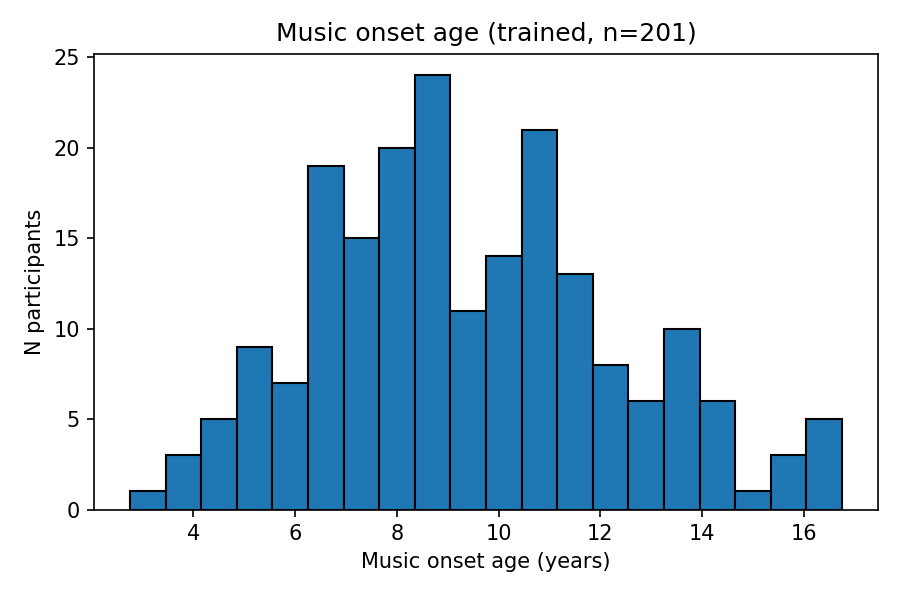
\includegraphics[width=0.62\textwidth]{figures/fig1_onset_distribution.png}
\caption{Distribution of estimated music onset age in the trained subsample ($n=201$).}
\label{fig:onset}
\end{figure}

\subsection{Brain $\to$ PSM (Step 4)}

Figure~\ref{fig:brainpsm} summarizes the standardized coefficients from the 11 separate covariate-adjusted regressions testing whether each white-matter graph feature predicted PSM. Among the 11 features, small-worldness showed the largest positive association with PSM ($\beta=+0.130$, raw $p=0.019$), followed by modularity. Several features had coefficients close to zero, whereas FPN within-network strength and characteristic path length showed negative coefficients. However, none of the associations survived FDR correction; all corrected $q$-values exceeded 0.21. Thus, Step 4 provides only a nominal brain--behavior signal rather than confirmatory evidence. The positive direction of small-worldness is nevertheless consistent with the idea that better episodic memory may be related to a more balanced integration--segregation profile in the developing structural connectome.

\begin{figure}[ht]
\centering
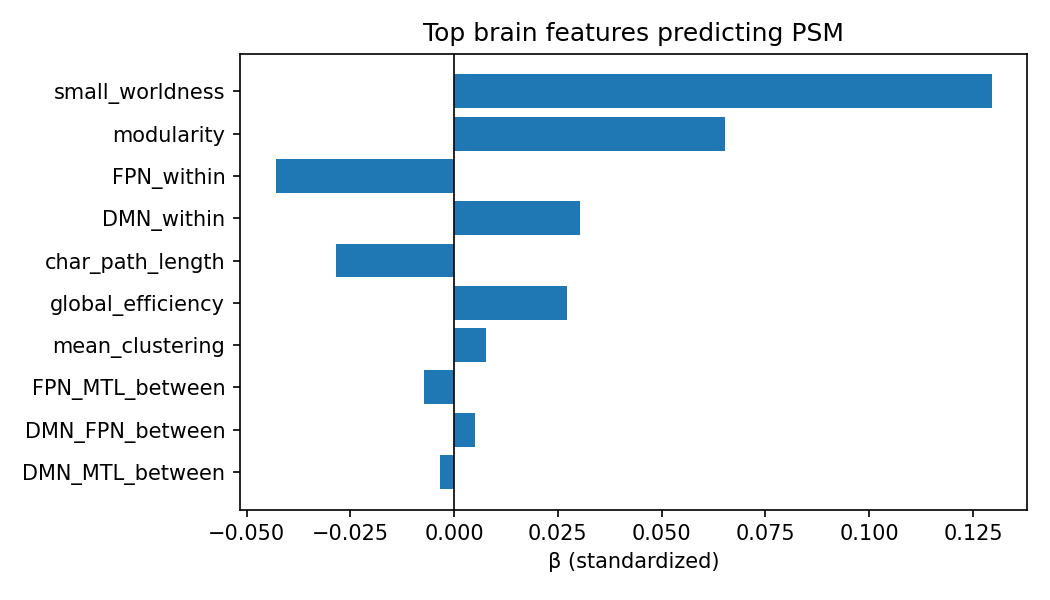
\includegraphics[width=0.70\textwidth]{figures/fig3_brain_behavior.png}
\caption{Standardized regression coefficients for each graph-theoretic feature predicting PSM in the Step 4 Brain $\to$ PSM analysis ($n=306$). Positive values indicate higher PSM with larger graph-feature values, whereas negative values indicate lower PSM. Small-worldness showed the largest nominal positive association, but all FDR-corrected $q$-values exceeded 0.21.}
\label{fig:brainpsm}
\end{figure}

\subsection{Music $\to$ PSM (Step 5)}

Before turning to the adjusted regression models, the raw group-level pattern shows why this analysis required a joint model. In the unadjusted boxplot, the late-onset group has a slightly higher median PSM score than the early- or middle-onset groups (Fig.~\ref{fig:rawpsm}). Taken at face value, this descriptive pattern appears inconsistent with a sensitive-period account. However, the raw comparison does not adjust for developmental and training-history differences. In HCP-D, later starters tend to be older, and older participants have more developmentally mature PSM performance. The raw plot therefore mixes onset timing with age and cumulative training history.

\begin{figure}[ht]
\centering
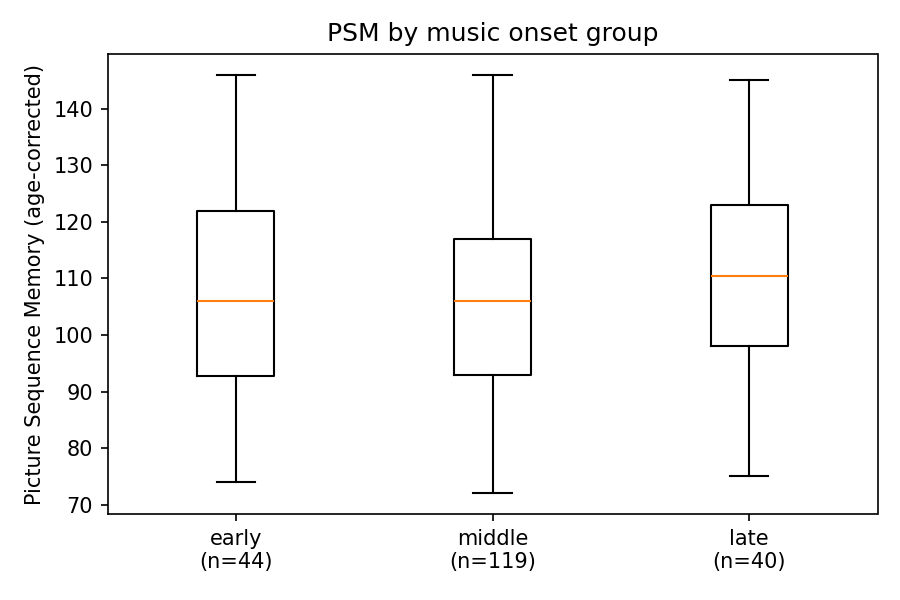
\includegraphics[width=0.62\textwidth]{figures/fig2_psm_by_group.png}
\caption{Raw, unadjusted PSM by music onset group. The late-onset group has a marginally higher median than the early-onset group, a pattern that reverses once cumulative hours and demographic covariates are controlled.}
\label{fig:rawpsm}
\end{figure}

The adjusted nested models clarify this reversal. In the marginal regressions, neither onset age alone (M1: $\beta=-0.092$, $p=0.30$) nor cumulative hours alone (M2: $\beta=-0.039$, $p=0.63$) reached significance. In the primary joint model M3, however, onset age became more strongly negative ($\beta=-0.207$, $p=0.073$), whereas cumulative hours remained smaller in magnitude ($\beta=-0.158$, $p=0.129$). Thus, once shared variance with cumulative hours was separated, the onset coefficient more than doubled in magnitude. The onset $\times$ hours interaction in M4 was effectively zero ($\beta=+0.030$, $p=0.742$), indicating that the pattern was additive rather than dependent on a training-hours threshold.

The headline result of the project is the comparison of M1, M2, and M3 (Table~\ref{tab:nested}, Fig.~\ref{fig:suppressor}). In M3, the absolute onset coefficient was larger than the absolute hours coefficient:
\[
\frac{|\beta_{\mathrm{onset}}|}{|\beta_{\mathrm{hours}}|}
=
\frac{0.207}{0.158}
\approx 1.31.
\]

\begin{table}[ht]
\centering
\caption{Standardized coefficients across nested music--PSM models. The trained-only subsample was used ($n\approx183$). M3 is the pre-registered primary model.}
\label{tab:nested}
\begin{tabular}{llrr}
\toprule
Model & Predictor & $\beta$ & $p$ \\
\midrule
M1 (onset only)      & onset age             & $-0.092$ & 0.300 \\
M2 (hours only)      & log hours             & $-0.039$ & 0.629 \\
\textbf{M3 (both)}   & \textbf{onset age}    & $\mathbf{-0.207}$ & 0.073 \\
\textbf{M3 (both)}   & \textbf{log hours}    & $\mathbf{-0.158}$ & 0.129 \\
M4 ($+$ interaction) & onset age             & $-0.215$ & 0.070 \\
M4 ($+$ interaction) & log hours             & $-0.160$ & 0.126 \\
M4 ($+$ interaction) & onset $\times$ hours  & $+0.030$ & 0.742 \\
\bottomrule
\end{tabular}
\end{table}

\begin{figure}[ht]
\centering
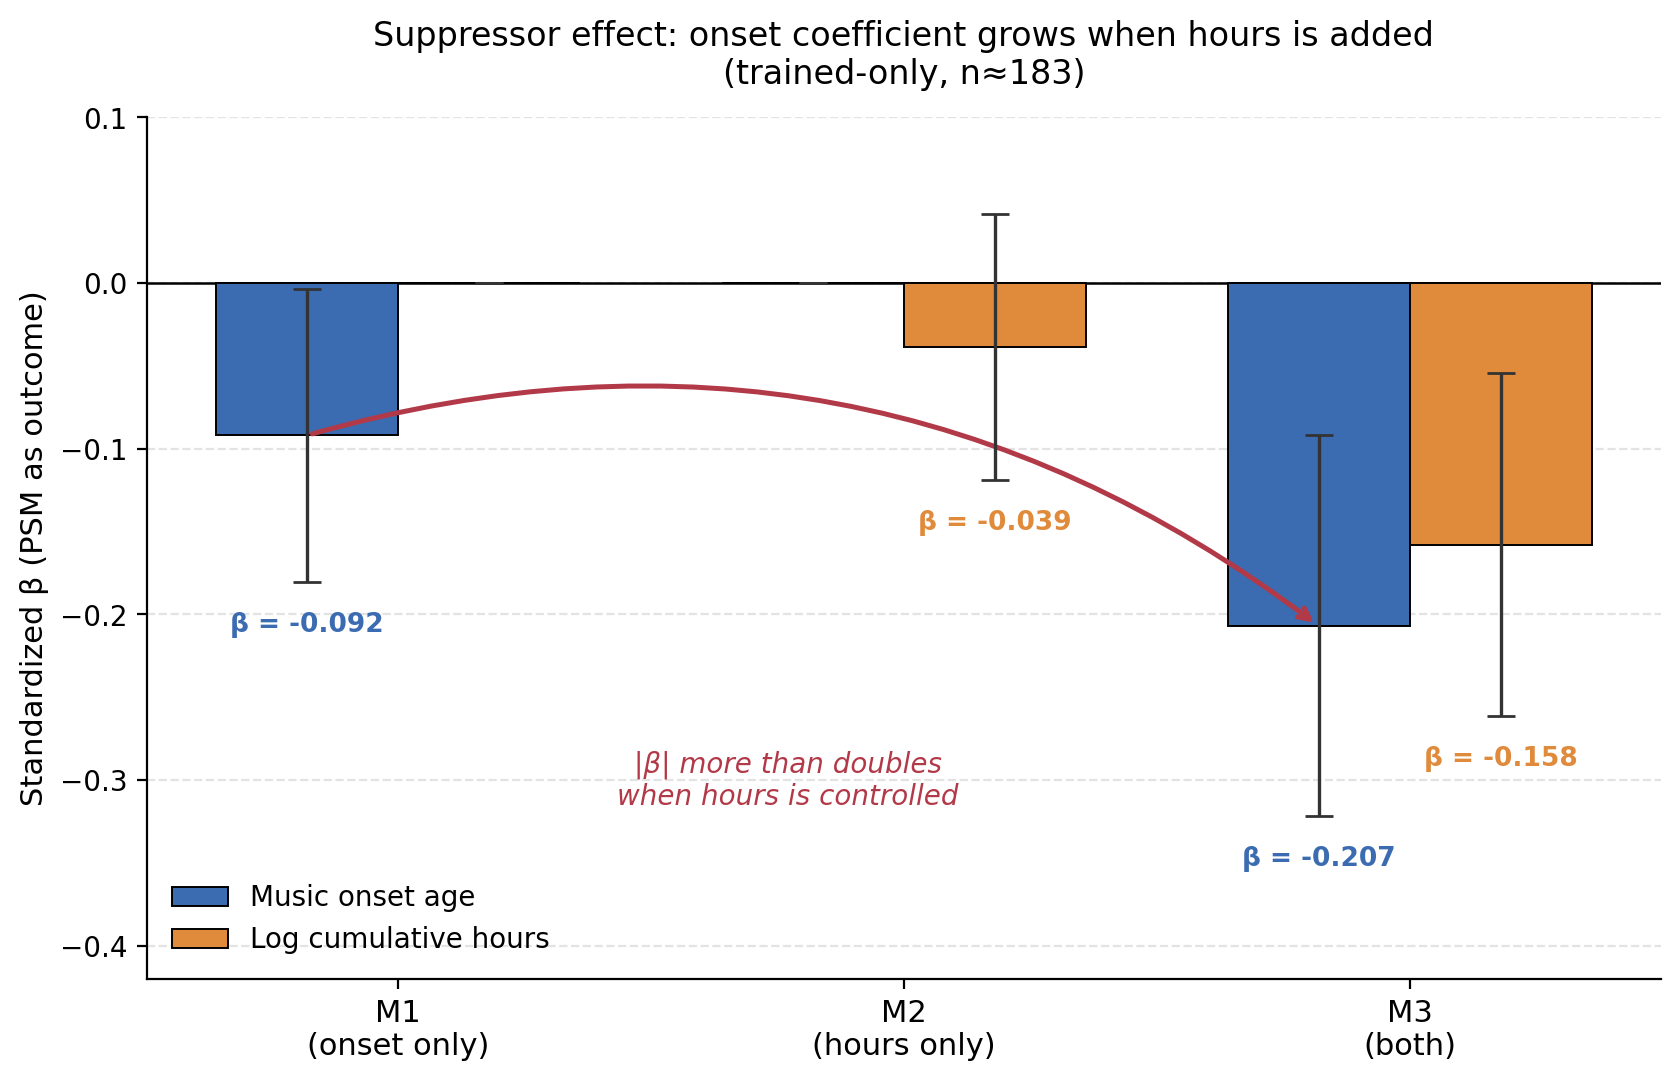
\includegraphics[width=0.70\textwidth]{figures/fig5_suppressor.png}
\caption{Suppressor pattern across the M1, M2, M3 nested model sequence. Error bars are $\pm 1$ SE. The curve traces the growth in onset's coefficient from $-0.092$ in M1, the marginal model, to $-0.207$ in M3, the partial model.}
\label{fig:suppressor}
\end{figure}

This pattern is diagnostic. A pure dose-response account would predict that the hours coefficient should be the larger coefficient once both predictors are entered, and that it should be positive. Instead, the relative ordering was the opposite: the onset coefficient was larger in magnitude than the hours coefficient, with
\[
\frac{|\beta(\mathrm{onset})|}{|\beta(\mathrm{hours})|}
=
\frac{0.207}{0.158}
\approx 1.31.
\]
The negative onset coefficient is consistent with the sensitive-period prediction that later onset is associated with lower PSM. By contrast, the negative hours coefficient does not support a positive dose-response interpretation. The interaction's near-zero value further rules out the sub-hypothesis that the onset effect depends on having reached some cumulative training threshold.

In M3, onset age and log cumulative hours were weakly negatively correlated ($r=-0.27$), but their variance inflation factors were 2.37 and 2.14, respectively, well below the conventional threshold of 5. The observed suppressor effect therefore reflects the separation of the two predictors' partial effects once their shared variance is controlled, rather than estimation instability arising from multicollinearity.

Overall, the M3 pattern is directionally consistent with H1a: onset age had the larger absolute partial coefficient, and its sign was negative. However, because neither coefficient reached conventional significance, this result should be interpreted as exploratory support for an onset-dominant pattern rather than confirmatory evidence for a sensitive-period effect.

\subsubsection{Secondary cognitive outcomes: specificity of the effect}

To test whether the PSM effect is specific to episodic memory or instead reflects a broader effect across general cognition, the same nested models were repeated for four secondary cognitive outcomes: Flanker (inhibitory control), DCCS (cognitive flexibility / set-shifting), List Sorting Working Memory, and Pattern Comparison Processing Speed. These analyses were conducted in the trained-only subsample ($n=183$). Table~\ref{tab:secondary_outcomes} summarizes the standardized partial coefficients of onset age and log cumulative hours from the primary joint model M3 for each outcome.

\begin{table}[ht]
\centering
\caption{Standardized partial regression coefficients from M3, in which onset age and log cumulative hours were entered jointly. The trained-only subsample was used ($n=183$). PSM, the primary outcome, is included for comparison.}
\label{tab:secondary_outcomes}
\resizebox{\textwidth}{!}{%
\begin{tabular}{lrrrr}
\toprule
Outcome (domain) & onset $\beta$ & hours $\beta$ & onset $p$ & $|\beta_{\text{onset}}|/|\beta_{\text{hours}}|$ \\
\midrule
\textbf{PSM} (episodic memory, reference) & \textbf{$-0.207$} & $-0.158$ & $0.073$ & $1.31$ \\
DCCS (cognitive flexibility) & $-0.232$ & $-0.015$ & $0.054$ & $15.0$ \\
List Sorting (working memory) & $-0.189$ & $-0.141$ & $0.119$ & $1.34$ \\
Pattern Comparison (processing speed) & $-0.122$ & $+0.054$ & $0.288$ & $2.28$ \\
Flanker (inhibitory control) & $-0.043$ & $+0.128$ & $0.720$ & $0.34$ \\
\bottomrule
\end{tabular}%
}
\end{table}

No secondary outcome survived FDR correction, and the trained-only sample ($n=183$) is small for multivariate regression. The interpretation below is therefore exploratory: it describes the effect-size pattern rather than providing a confirmatory claim. Even so, two regularities are worth noting. First, onset's partial effect was larger than hours' partial effect in three of the four secondary outcomes: DCCS, List Sorting, and Pattern Comparison. This suggests that the suppressor/sensitive-period pattern observed for PSM in Section~4.3 is not simply an artifact of a single outcome. The onset coefficient for DCCS in particular ($\beta=-0.232$, $p=0.054$) was larger than that for PSM ($\beta=-0.207$) and approached nominal significance.

Second, the magnitude of the onset signal varied systematically by domain. It was strongest for tasks involving sequencing, memory, and executive control, namely PSM, DCCS, and List Sorting, but weaker or absent for lower-level processing speed and simple inhibition. Flanker was the sole exception, and was the only outcome for which hours showed a larger coefficient than onset. This gradient is consistent with a near-transfer interpretation. In this interpretation, the trace of music onset is concentrated in cognitive domains closely related to the demands of music learning, such as sequencing, memory, and working control, and is weaker in domains that share less structure with music training. This pattern fits a selective sensitive-period account better than a skeptical account in which the apparent music effect is merely a uniform lift in general cognitive ability. Because all coefficients were FDR-nonsignificant and the trained-only sample was modest, however, this interpretation should be treated as a hypothesis for future work rather than as a definitive conclusion.

\subsection{Music $\to$ Brain (Step 6)}

Twenty-two regressions were estimated: 11 graph features $\times$ 2 music predictors. None survived FDR correction. The most prominent raw signals were DMN--FPN between-network connectivity with log cumulative hours ($\beta=+0.13$, $p=0.25$) and small-worldness with onset age ($\beta=-0.13$, $p=0.28$). Both effects were too weak to interpret individually, but their directions were broadly consistent with the hypothesized pattern: more practice was associated with stronger between-network connectivity, whereas later onset was associated with less small-world structure.

\subsection{Mediation: Onset $\to$ Brain $\to$ PSM (Step 7)}

Across all 11 candidate mediators, the bootstrap 95\% confidence intervals for the indirect effect ($a \times b$) included zero (Fig.~\ref{fig:mediation}). The largest point estimate was observed for small-worldness ($a \times b=-0.016$, CI $[-0.063, +0.020]$, $p_{\text{boot}}=0.40$). Its direction was consistent with the sensitive-period prediction, but the indirect effect was statistically null.

\begin{figure}[ht]
\centering
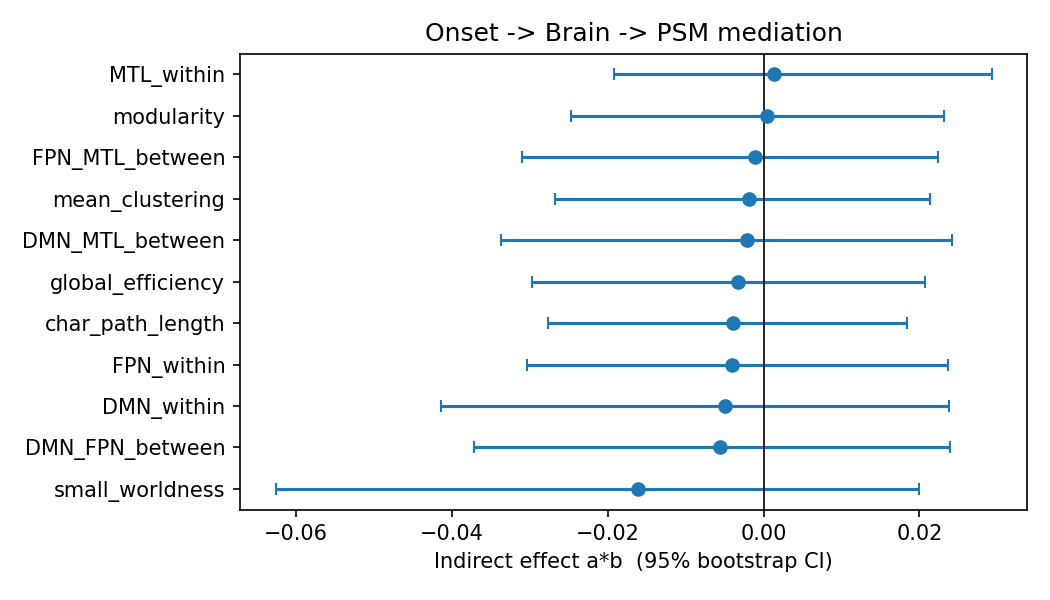
\includegraphics[width=0.72\textwidth]{figures/fig4_mediation.png}
\caption{Indirect effects of music onset age on PSM through each of the 11 candidate white-matter mediators. Whiskers indicate 95\% bootstrap confidence intervals based on 5{,}000 resamples. All intervals include zero.}
\label{fig:mediation}
\end{figure}

Importantly, the direct effect of onset age on PSM, corresponding to the $c$-path ($\beta=-0.236$), was only minimally attenuated to $c' \approx -0.22$ in every mediator-specific model. This indicates that the onset age $\to$ PSM association does not pass through the macroscale white-matter graph features tested here.




% ==================================================================
\section{Discussion}

\subsection{Verdict on the three scenarios}

The \textbf{sensitive-period scenario} is the best-fitting of the three pre-registered hypotheses, but only weakly. The main support comes from the primary joint model M3: onset age had a larger absolute partial coefficient than cumulative hours, and the onset coefficient was negative, as predicted by H1a. This means that later music onset was associated with lower PSM after cumulative hours and covariates were controlled. However, this support is qualified by two facts. First, neither coefficient reached $p<0.05$, with the primary onset coefficient sitting in the marginal $p\approx0.07$ range. Second, the macroscale mediation pathway was empirically absent. Thus, if a sensitive-period effect is present in this sample, it does not appear to operate through the eleven topology features measured here.

The \textbf{dose-response scenario} is weakly disfavored. A pure dose-response account would predict that cumulative hours should be the stronger predictor and that its coefficient should be positive. Instead, after onset age was held constant, the hours coefficient was smaller in magnitude than the onset coefficient and was negative. The interaction was also null, so there was no evidence that high-dose training amplified an onset effect.

The \textbf{skeptical scenario cannot be confidently rejected}: nothing survives FDR correction, the trained-only sample ($n=183$) is modest for a multi-predictor regression, and---critically---our covariate set (age, sex, fluid reasoning) does not include socioeconomic status or family-environment measures, the very confounders emphasized by the skeptical account. We therefore cannot rule out that the onset pattern partly reflects unmeasured background variables.


\subsection{Why the macroscale connectome may be silent}
The most informative negative result is the mediation null. \citet{steele2013} localized their sensitive-period effect to the posterior corpus callosum, using fractional anisotropy from tractography---a microstructural and tract-specific measure. Our 11 features are by contrast network-level summaries of the whole-brain graph after thresholding. Two interpretations are plausible:
\begin{itemize}[leftmargin=1.4em,itemsep=2pt]
  \item \textbf{Wrong spatial scale.} A localized FA difference in a specific commissural tract may not change network-level topology metrics like small-worldness or modularity. The signal could be there at the tract level and invisible at the global level.
  \item \textbf{Wrong tissue.} Sequence memory depends critically on hippocampal--prefrontal circuitry. Gray-matter volume in MTL or functional connectivity between MTL and FPN may be a more direct substrate than aggregate structural-connectome topology.
\end{itemize}
Either way, the appropriate next experiment is not a larger-$N$ replication of the same pipeline; it is a redesign with tract-specific microstructural metrics (FA, RD) in tracts of interest, or with hippocampal/MTL volumetry, applied to the same HCP-D sample.

\subsection{Connection to the lifespan turning-points framework}
The single nominally-significant Brain $\to$ PSM signal---small-worldness, $\beta=+0.13$---is not arbitrary. \citet{mousley2025} reported that small-worldness has the largest LASSO coefficient for predicting age in the 9--32 lifespan epoch, the epoch that contains the entire HCP-D age range. That our only behavioral hit is in the same metric the lifespan paper flags as the dominant developmental axis in this age window is at least consistent with the idea that PSM-relevant connectome reorganization in this epoch operates partly through small-worldness. This is a hypothesis the present study cannot resolve---it survives as a finding to follow up.

\subsection{Limitations}
\begin{itemize}[leftmargin=1.4em,itemsep=2pt]
  \item \textbf{Power.} Trained-only $n=183$. The primary M3 onset coefficient sits at $p=0.07$, in the uncomfortable zone where adding 50--100 participants would likely settle the question one way or the other.
  \item \textbf{Onset coverage.} Only $\approx22\%$ of trained participants started before age 7. The classical Steele-style contrast is underpowered by sample composition, not by sample size.
  \item \textbf{Unmeasured confounders.} No socioeconomic-status or family-income covariate was available in the analysis sample, so the skeptical scenario cannot be fully addressed.
  \item \textbf{Self-report.} Music history is retrospective parental/self-report, and cumulative hours is estimated from coarse multiplicative units that compound measurement noise.
  \item \textbf{Cross-sectional.} Causal direction cannot be separated---``better brain $\to$ earlier start'' remains formally indistinguishable from ``earlier start $\to$ better brain.''
  \item \textbf{Macroscale features only.} We did not test tract-specific FA/RD, gray-matter volume, or functional connectivity, any of which could carry the trace that macroscale topology does not.
\end{itemize}

% ==================================================================
\section{Conclusion}
This project asked whether the timing of musical onset leaves a detectable trace in episodic memory and in the macroscale white-matter connectome. Using a pre-registered three-scenario framework, I found: (i) \emph{behavior}---a textbook suppressor pattern in which onset's partial effect on PSM grows from $|\beta|=0.09$ to $|\beta|=0.21$ when cumulative hours is controlled, and is larger in magnitude than hours' partial effect ($p=0.073$, $n=183$), the signature predicted by the sensitive-period scenario; (ii) \emph{brain}---only small-worldness predicts PSM at the nominal level (raw $p=0.019$, FDR n.s.), the same metric lifespan work \citep{mousley2025} identifies as the strongest age predictor for the 9--32 epoch our sample sits in; and (iii) \emph{mediation}---no macroscale topology feature carries the onset $\to$ PSM signal (all 11 indirect-effect 95\% CIs include zero). The honest summary is that the data lean toward the sensitive-period scenario in behavior, but the trace, if real, is not in macroscale white-matter topology. The most productive next step is to redirect the search toward tract-specific microstructure and toward MTL gray-matter and functional measures---exactly the substrates where the original sensitive-period and episodic-memory literatures locate the relevant biology.

% ==================================================================
\begin{thebibliography}{9}
\bibitem[Bigand \& Tillmann(2022)]{bigand2022} Bigand, E., \& Tillmann, B. (2022). Near and far transfer: Is music special? \emph{Memory \& Cognition, 50}(2), 339--347.
\bibitem[Mousley et al.(2025)]{mousley2025} Mousley, A., Bethlehem, R. A. I., Yeh, F.-C., \& Astle, D. E. (2025). Topological turning points across the human lifespan. \emph{Nature Communications, 16}, 10055.
\bibitem[Sala \& Gobet(2017)]{sala2017} Sala, G., \& Gobet, F. (2017). When the music's over: Does music skill transfer to children's and young adolescents' cognitive and academic skills? A meta-analysis. \emph{Educational Research Review, 20}, 55--67.
\bibitem[Schellenberg(2020)]{schellenberg2020} Schellenberg, E. G. (2020). Correlation $=$ causation? Music training, psychology, and neuroscience. \emph{Psychology of Aesthetics, Creativity, and the Arts, 14}(4), 475--480.
\bibitem[Steele et al.(2013)]{steele2013} Steele, C. J., Bailey, J. A., Zatorre, R. J., \& Penhune, V. B. (2013). Early musical training and white-matter plasticity in the corpus callosum: Evidence for a sensitive period. \emph{Journal of Neuroscience, 33}(3), 1282--1290.
\end{thebibliography}


\end{document}
